%!TEX program = xelatex

\documentclass[cn,black,9pt,normal]{elegantnote}
\usepackage{float}
\usepackage{hyperref}


%\newcommand{\upcite}[1]{\textsuperscript{\textsuperscript{\cite{#1}}}}

\title{数码摄影作业(04)两张自然景物的照片\\\small{花花草草}}
\author{姓名:姜文渊\\学号:1951510}
%\institute{School of Life Science, Tongji University}
%\version{1.00}
\date{2021年4月5日}

\begin{document}

\maketitle


\section*{拍摄条件及使用器材简介}

作业中使用的相机为佳能M200。第一张照片摄于笔者老家兴化的油菜田里,使用的镜头为\texttt{EF-M15-45mm f/3.5-6.3 IS STM},加装了某国产偏振镜。
第二张照片摄于同济大学图书馆前的草坪,使用的镜头为\texttt{TTArtisan 50mm f1.2}。

\section{所摄照片}
\begin{figure}[H]
    \centering
    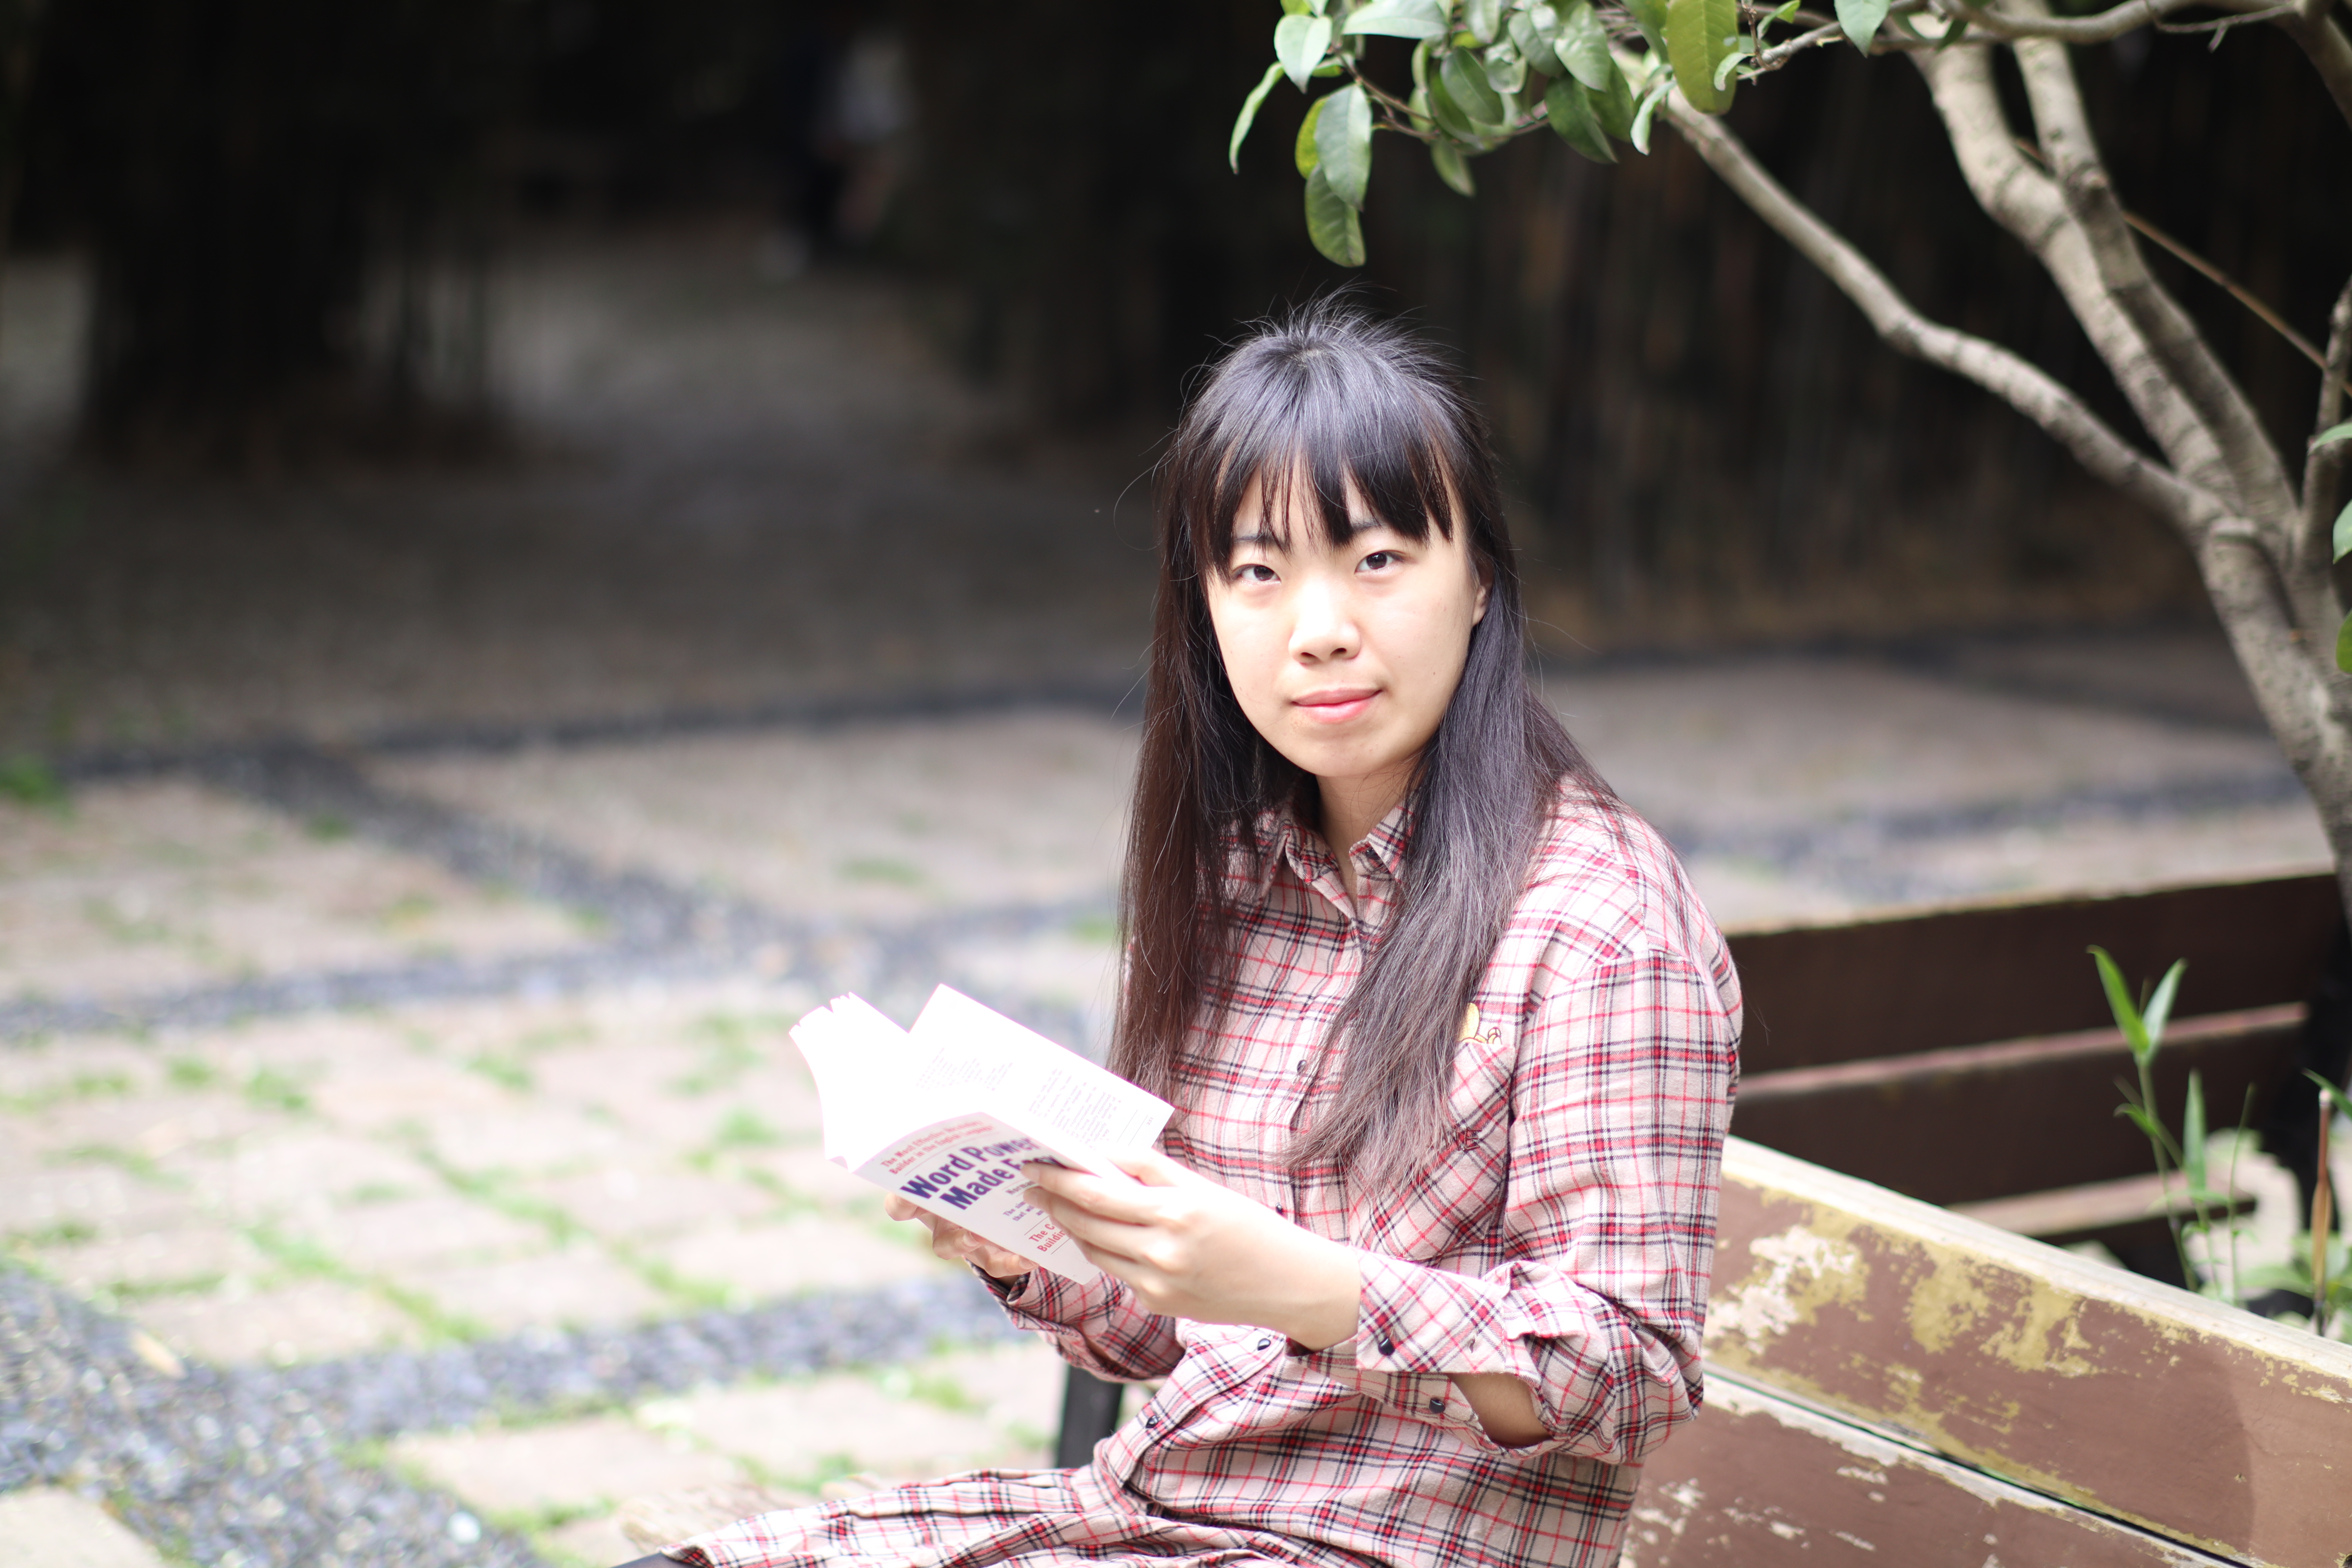
\includegraphics[width=0.9\textwidth]{F1.JPG}
    \caption{28mm 1/2000 F5.0 ISO 100}
    \label{F-01}
\end{figure}

上面的照片使用三分之一布局,油菜花占据下三分之二,天空占据上三分之一,意在表现春日油菜花盛开的生机勃勃之景象。
油菜花田作为笔者家乡的特色,常常以被俯视的角度拍摄,而这张照片以从与油菜花齐平的高度拍摄,更能给人以身临其境的感受。

\section{所摄照片}
\begin{figure}[H]
    \centering
    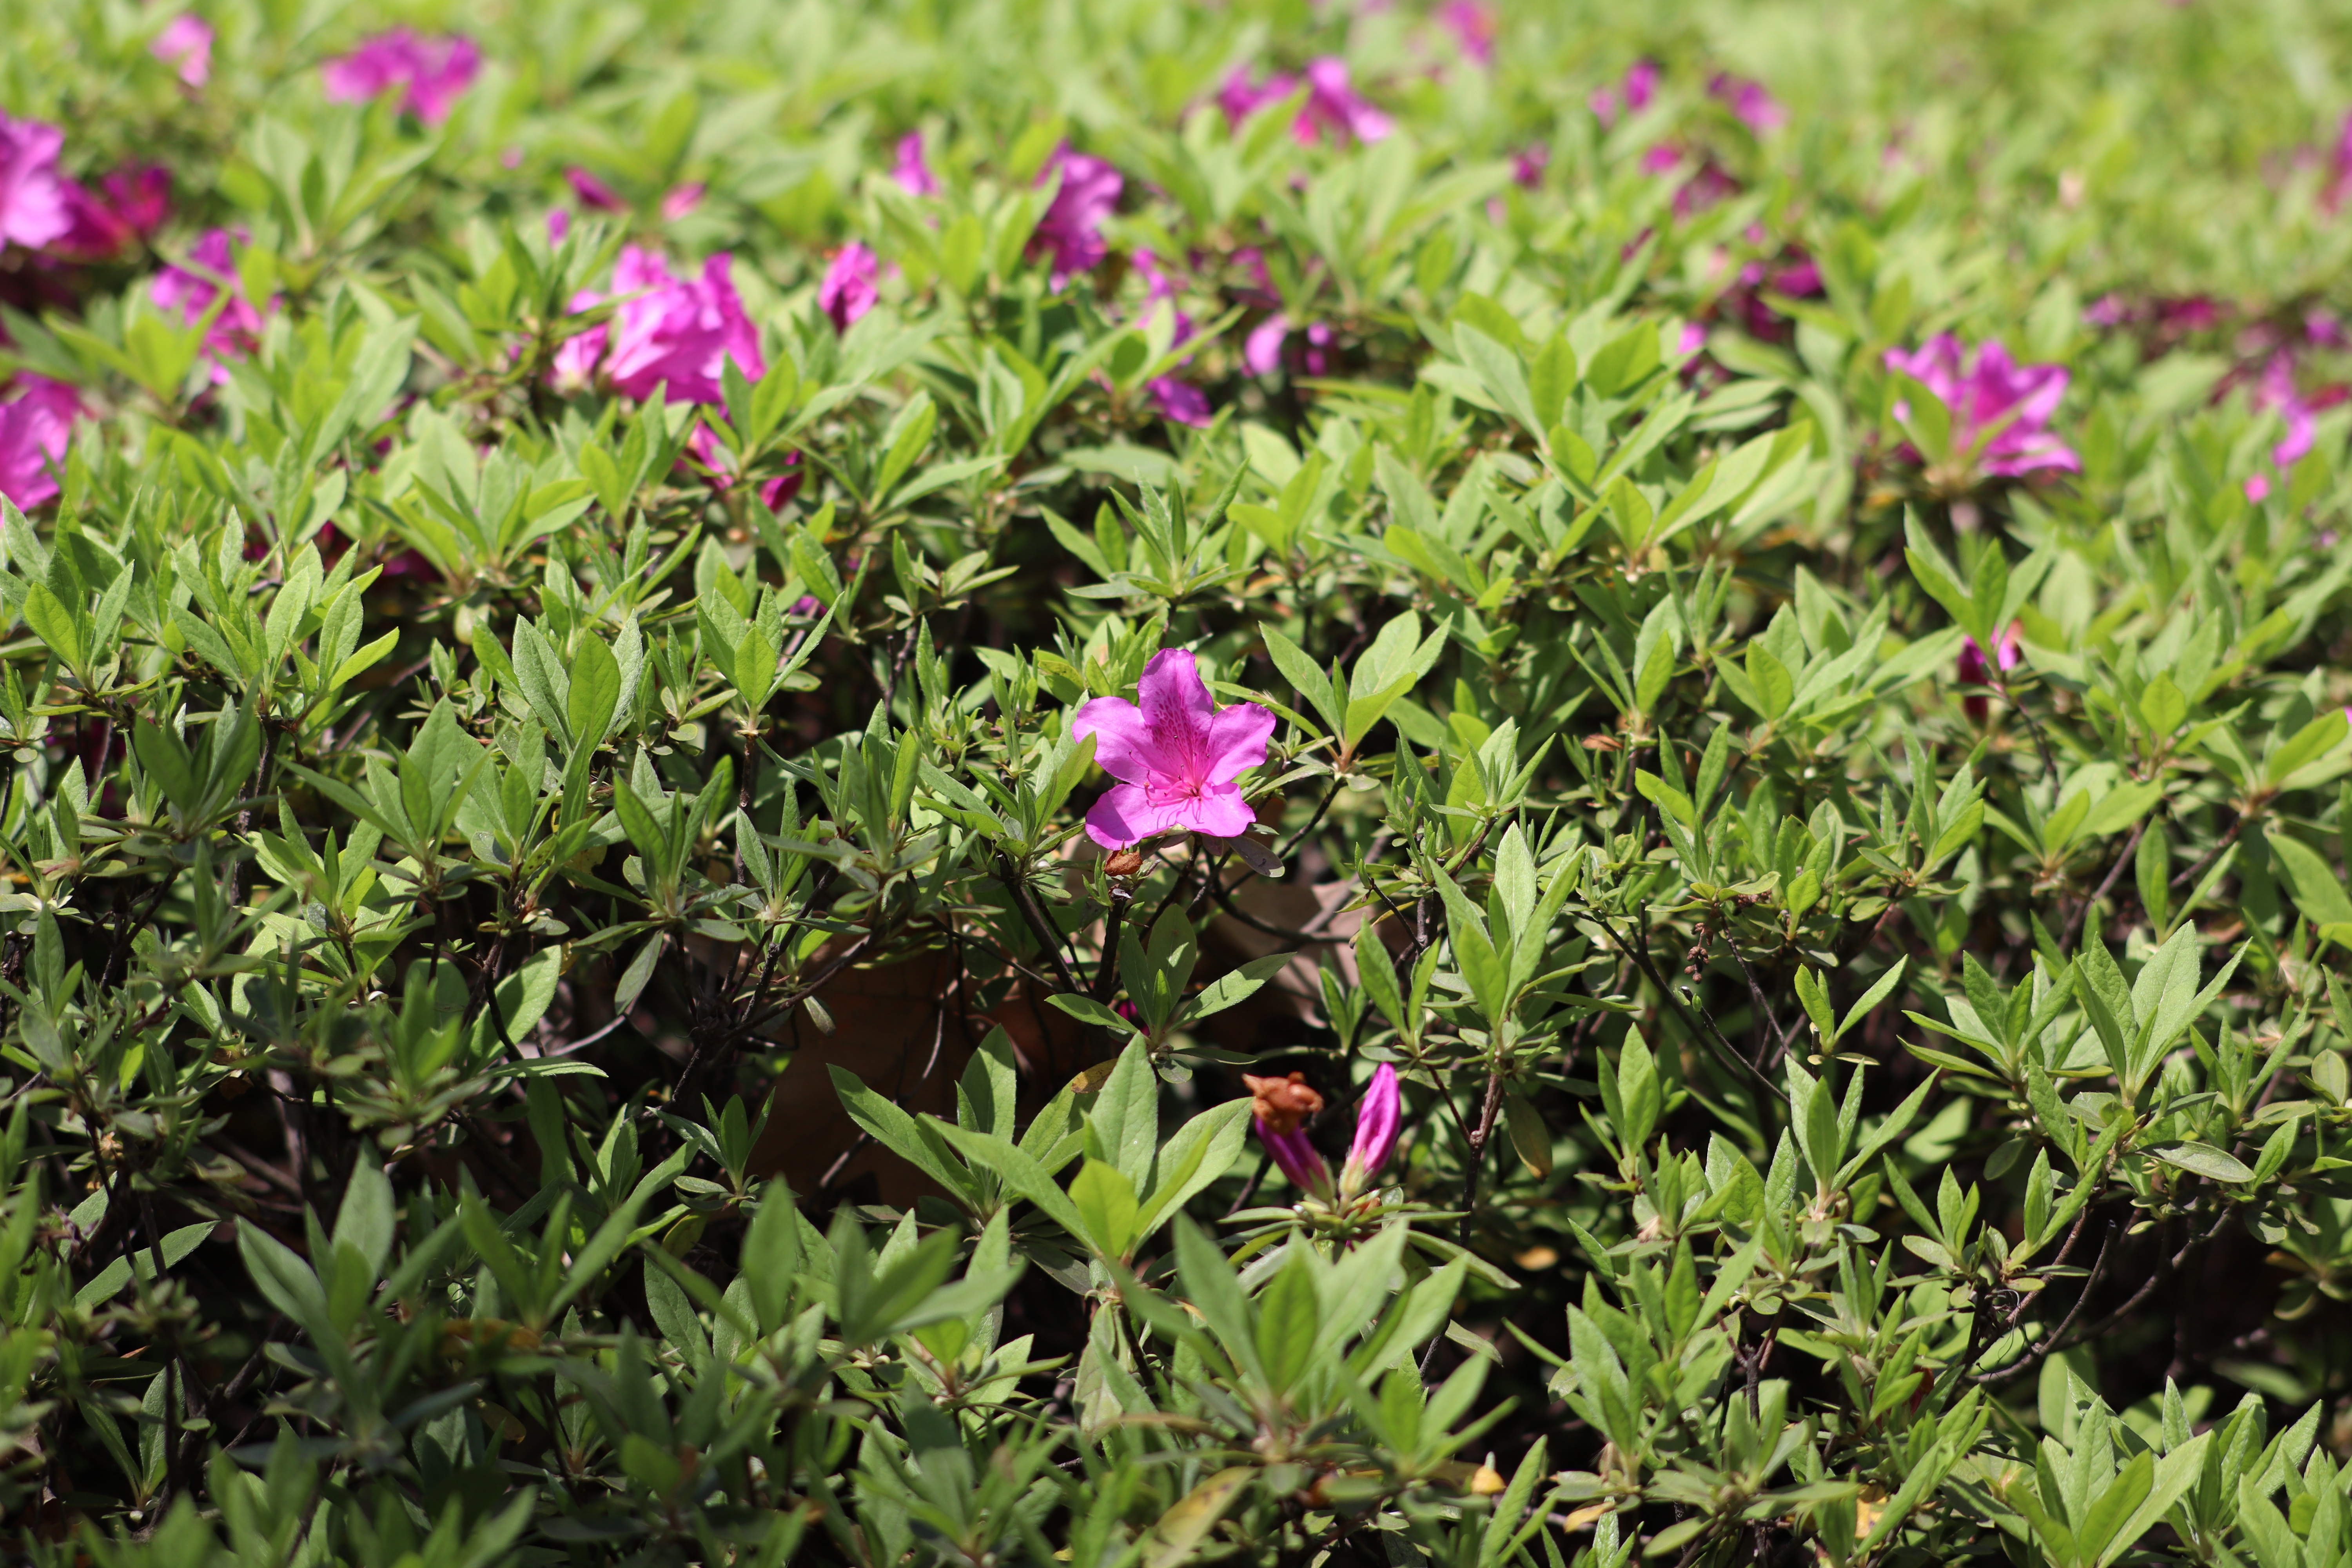
\includegraphics[width=1\textwidth]{F2.JPG}
    \caption{50mm 1/2000 F2.0 ISO 100}
    \label{F-02}
\end{figure}

这张照片是笔者在图书馆门前的绿化带中拍摄的照片,使用的是一手动定焦镜头,所摄主体位于照片中央,颜色对比鲜明,
后面的花朵因为不处于焦平面内,故而呈现虚化的效果,更加突出画面中央的花朵的重要性。
%\bibstyle{unsrt}
%\bibliography{references}{}
\end{document}
